% Kapitel 1
% Die Unterkapitel können auch in separaten Dateien stehen,
% die dann mit dem \include-Befehl eingebunden werden.
%-------------------------------------------------------------------------------

\chapter{Einleitung}
%Hier Einleitungstext einfügen, dabei die Formatierungen selber erstellen
Hier ist die Arbeitsweise des Systems anhand von State-Charts darzustellen und
kurz zu erläutern.
\section{Projektdetails}
Die Details der Aufgabenstellung bitte anhand von Statecharts darstellen und
kurz verbal beschreiben.

\section{GUI}
Über das GUI soll der Anwender in der Lage sein, dass Programm mit allen vorhandenen Funktionen zu bedienen.
Nach dem Programmstart befindet sich der Anwender in einem Initialzustand. Hierbei sind die Felder des 2D-Modells und der 3D-Darstellung noch leer und die Physikparameter haben Ihre Initialwerte. Man ist in der Lage die Konstruktionsdaten aus dem Editor zu laden um die Bahn erstellen zu können.
Ist dies geschehen, befindet sich der Anwender in der Vorschau. Hier wird ein 2D-Modell der Bahn angezeigt und es können noch Änderungen an den Grafikeinstellungen, sowie den Physikparametern vorgenommen werden. Das Feld der 3D-Darstellung ist weiterhin leer. Aus der Vorschau heraus kann nun auch die Simulation gestartet werden.
Wurde die Simulation gestartet, erscheint sie in dem dafür vorgesehenem Feld. Bei Bedarf kann sie auf Bildschirmgröße maximiert werden. Während der laufenden Simulation können die Simulationsparameter angepasst werden.
Wird die Simulation gestoppt, befindet man sich wieder in der Vorschau, von wo aus man mit dem Schließen der Konstruktion wieder in den Initialzustand gelangt.
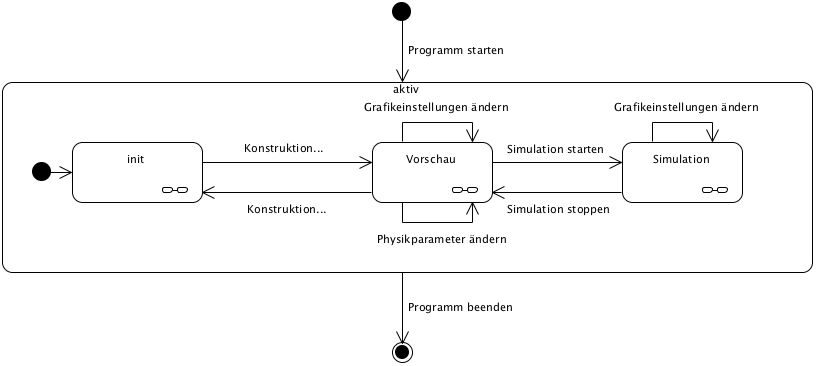
\includegraphics[width=16cm]{bilder/StateChart_GUI}
